\documentclass{standalone}
\usepackage{tikz}
\usetikzlibrary{patterns, positioning}

\begin{document}
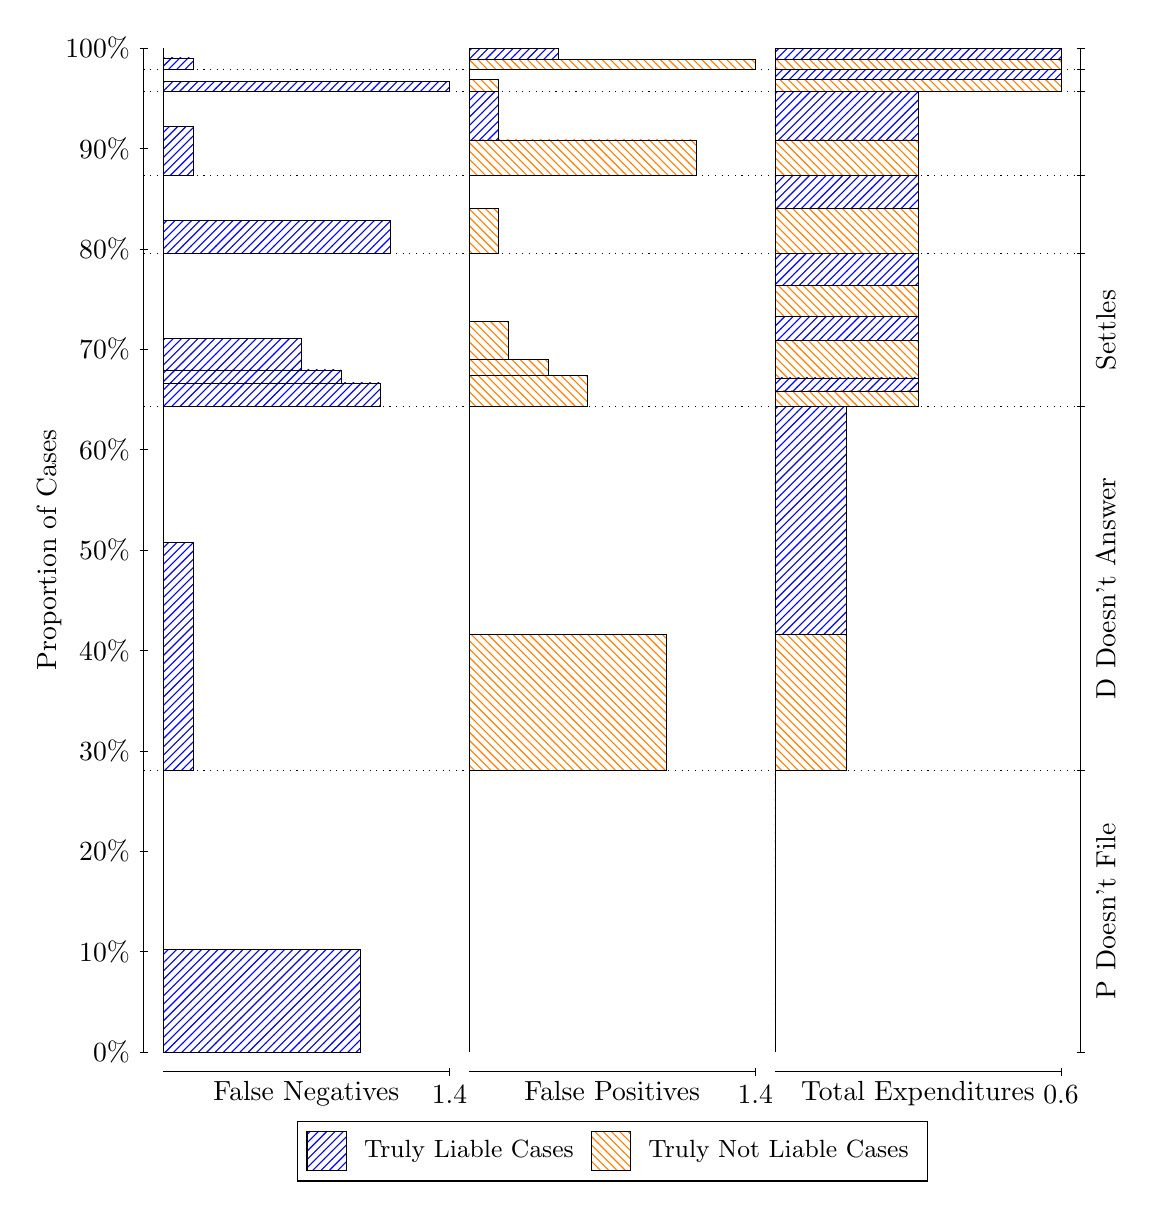
\begin{tikzpicture}
\draw[black, very thin] (1.5,1.75) -- (1.5,14.5);
\node[rotate=90, anchor=center] at (0.3, 8.125) {Proportion of Cases};
\draw[black, very thin] (1.45,1.75) -- (1.55,1.75);
\node[anchor=east] at (1.45, 1.75) {0\%};
\draw[black, very thin] (1.45,3.025) -- (1.55,3.025);
\node[anchor=east] at (1.45, 3.025) {10\%};
\draw[black, very thin] (1.45,4.3) -- (1.55,4.3);
\node[anchor=east] at (1.45, 4.3) {20\%};
\draw[black, very thin] (1.45,5.575) -- (1.55,5.575);
\node[anchor=east] at (1.45, 5.575) {30\%};
\draw[black, very thin] (1.45,6.85) -- (1.55,6.85);
\node[anchor=east] at (1.45, 6.85) {40\%};
\draw[black, very thin] (1.45,8.125) -- (1.55,8.125);
\node[anchor=east] at (1.45, 8.125) {50\%};
\draw[black, very thin] (1.45,9.4) -- (1.55,9.4);
\node[anchor=east] at (1.45, 9.4) {60\%};
\draw[black, very thin] (1.45,10.675) -- (1.55,10.675);
\node[anchor=east] at (1.45, 10.675) {70\%};
\draw[black, very thin] (1.45,11.95) -- (1.55,11.95);
\node[anchor=east] at (1.45, 11.95) {80\%};
\draw[black, very thin] (1.45,13.225) -- (1.55,13.225);
\node[anchor=east] at (1.45, 13.225) {90\%};
\draw[black, very thin] (1.45,14.5) -- (1.55,14.5);
\node[anchor=east] at (1.45, 14.5) {100\%};

\draw[black, very thin] (13.4,1.75) -- (13.4,14.5);
\draw[black, very thin] (13.35,1.75) -- (13.45,1.75);
\node[anchor=west] at (13.35, 1.75) {};
\draw[black, very thin] (13.35,5.3283) -- (13.45,5.3283);
\node[anchor=west] at (13.35, 5.3283) {};
\draw[black, very thin] (13.35,9.9485) -- (13.45,9.9485);
\node[anchor=west] at (13.35, 9.9485) {};
\draw[black, very thin] (13.35,11.888) -- (13.45,11.888);
\node[anchor=west] at (13.35, 11.888) {};
\draw[black, very thin] (13.35,12.883) -- (13.45,12.883);
\node[anchor=west] at (13.35, 12.883) {};
\draw[black, very thin] (13.35,13.951) -- (13.45,13.951);
\node[anchor=west] at (13.35, 13.951) {};
\draw[black, very thin] (13.35,14.228) -- (13.45,14.228);
\node[anchor=west] at (13.35, 14.228) {};
\draw[black, very thin] (13.35,14.5) -- (13.45,14.5);
\node[anchor=west] at (13.35, 14.5) {};

\draw[black, very thin, pattern color=blue, pattern=north east lines] (1.75,1.75) rectangle (4.2557,3.0543);
\draw[black, very thin, pattern color=orange, pattern=north west lines] (1.75,3.0543) rectangle (1.75,5.3283);
\draw[black, very thin, pattern color=blue, pattern=north east lines] (1.75,5.3283) rectangle (2.1259,8.2231);
\draw[black, very thin, pattern color=orange, pattern=north west lines] (1.75,8.2231) rectangle (1.75,9.9485);
\draw[black, very thin, pattern color=blue, pattern=north east lines] (1.75,9.9485) rectangle (4.5063,10.247);
\draw[black, very thin, pattern color=blue, pattern=north east lines] (1.75,10.247) rectangle (4.0052,10.413);
\draw[black, very thin, pattern color=blue, pattern=north east lines] (1.75,10.413) rectangle (3.504,10.812);
\draw[black, very thin, pattern color=orange, pattern=north west lines] (1.75,10.812) rectangle (1.75,11.888);
\draw[black, very thin, pattern color=blue, pattern=north east lines] (1.75,11.888) rectangle (4.6316,12.309);
\draw[black, very thin, pattern color=orange, pattern=north west lines] (1.75,12.309) rectangle (1.75,12.883);
\draw[black, very thin, pattern color=blue, pattern=north east lines] (1.75,12.883) rectangle (2.1259,13.5);
\draw[black, very thin, pattern color=orange, pattern=north west lines] (1.75,13.5) rectangle (1.75,13.951);
\draw[black, very thin, pattern color=blue, pattern=north east lines] (1.75,13.951) rectangle (5.3833,14.077);
\draw[black, very thin, pattern color=orange, pattern=north west lines] (1.75,14.077) rectangle (1.75,14.228);
\draw[black, very thin, pattern color=blue, pattern=north east lines] (1.75,14.228) rectangle (2.1259,14.376);
\draw[black, very thin, pattern color=orange, pattern=north west lines] (1.75,14.376) rectangle (1.75,14.5);
\draw[black, very thin, pattern color=orange, pattern=north west lines] (5.6333,1.75) rectangle (5.6333,4.024);
\draw[black, very thin, pattern color=blue, pattern=north east lines] (5.6333,4.024) rectangle (5.6333,5.3283);
\draw[black, very thin, pattern color=orange, pattern=north west lines] (5.6333,5.3283) rectangle (8.1391,7.0537);
\draw[black, very thin, pattern color=blue, pattern=north east lines] (5.6333,7.0537) rectangle (5.6333,9.9485);
\draw[black, very thin, pattern color=orange, pattern=north west lines] (5.6333,9.9485) rectangle (7.1368,10.346);
\draw[black, very thin, pattern color=orange, pattern=north west lines] (5.6333,10.346) rectangle (6.6356,10.544);
\draw[black, very thin, pattern color=orange, pattern=north west lines] (5.6333,10.544) rectangle (6.1345,11.024);
\draw[black, very thin, pattern color=blue, pattern=north east lines] (5.6333,11.024) rectangle (5.6333,11.888);
\draw[black, very thin, pattern color=orange, pattern=north west lines] (5.6333,11.888) rectangle (6.0092,12.461);
\draw[black, very thin, pattern color=blue, pattern=north east lines] (5.6333,12.461) rectangle (5.6333,12.883);
\draw[black, very thin, pattern color=orange, pattern=north west lines] (5.6333,12.883) rectangle (8.5149,13.334);
\draw[black, very thin, pattern color=blue, pattern=north east lines] (5.6333,13.334) rectangle (6.0092,13.951);
\draw[black, very thin, pattern color=orange, pattern=north west lines] (5.6333,13.951) rectangle (6.0092,14.102);
\draw[black, very thin, pattern color=blue, pattern=north east lines] (5.6333,14.102) rectangle (5.6333,14.228);
\draw[black, very thin, pattern color=orange, pattern=north west lines] (5.6333,14.228) rectangle (9.2667,14.352);
\draw[black, very thin, pattern color=blue, pattern=north east lines] (5.6333,14.352) rectangle (6.7609,14.5);
\draw[black, very thin, pattern color=orange, pattern=north west lines] (9.5167,1.75) rectangle (9.5167,4.024);
\draw[black, very thin, pattern color=blue, pattern=north east lines] (9.5167,4.024) rectangle (9.5167,5.3283);
\draw[black, very thin, pattern color=orange, pattern=north west lines] (9.5167,5.3283) rectangle (10.425,7.0537);
\draw[black, very thin, pattern color=blue, pattern=north east lines] (9.5167,7.0537) rectangle (10.425,9.9485);
\draw[black, very thin, pattern color=orange, pattern=north west lines] (9.5167,9.9485) rectangle (11.333,10.146);
\draw[black, very thin, pattern color=blue, pattern=north east lines] (9.5167,10.146) rectangle (11.333,10.312);
\draw[black, very thin, pattern color=orange, pattern=north west lines] (9.5167,10.312) rectangle (11.333,10.792);
\draw[black, very thin, pattern color=blue, pattern=north east lines] (9.5167,10.792) rectangle (11.333,11.09);
\draw[black, very thin, pattern color=orange, pattern=north west lines] (9.5167,11.09) rectangle (11.333,11.488);
\draw[black, very thin, pattern color=blue, pattern=north east lines] (9.5167,11.488) rectangle (11.333,11.888);
\draw[black, very thin, pattern color=orange, pattern=north west lines] (9.5167,11.888) rectangle (11.333,12.461);
\draw[black, very thin, pattern color=blue, pattern=north east lines] (9.5167,12.461) rectangle (11.333,12.883);
\draw[black, very thin, pattern color=orange, pattern=north west lines] (9.5167,12.883) rectangle (11.333,13.334);
\draw[black, very thin, pattern color=blue, pattern=north east lines] (9.5167,13.334) rectangle (11.333,13.951);
\draw[black, very thin, pattern color=orange, pattern=north west lines] (9.5167,13.951) rectangle (13.15,14.102);
\draw[black, very thin, pattern color=blue, pattern=north east lines] (9.5167,14.102) rectangle (13.15,14.228);
\draw[black, very thin, pattern color=orange, pattern=north west lines] (9.5167,14.228) rectangle (13.15,14.352);
\draw[black, very thin, pattern color=blue, pattern=north east lines] (9.5167,14.352) rectangle (13.15,14.5);
\draw[black, dotted] (1.5,5.3283) -- (13.4,5.3283);
\draw[black, dotted] (1.5,9.9485) -- (13.4,9.9485);
\draw[black, dotted] (1.5,11.888) -- (13.4,11.888);
\draw[black, dotted] (1.5,12.883) -- (13.4,12.883);
\draw[black, dotted] (1.5,13.951) -- (13.4,13.951);
\draw[black, dotted] (1.5,14.228) -- (13.4,14.228);
\draw[black, very thin] (1.75,1.5) -- (5.3833,1.5);
\node[anchor=north] at (3.5667, 1.5) {False Negatives};
\draw[black, very thin] (5.3833,1.45) -- (5.3833,1.55);
\node[anchor=north] at (5.3833, 1.45) {1.4};

\draw[black, very thin] (5.6333,1.5) -- (9.2667,1.5);
\node[anchor=north] at (7.45, 1.5) {False Positives};
\draw[black, very thin] (9.2667,1.45) -- (9.2667,1.55);
\node[anchor=north] at (9.2667, 1.45) {1.4};

\draw[black, very thin] (9.5167,1.5) -- (13.15,1.5);
\node[anchor=north] at (11.333, 1.5) {Total Expenditures};
\draw[black, very thin] (13.15,1.45) -- (13.15,1.55);
\node[anchor=north] at (13.15, 1.45) {0.6};

\node[black, centered, rotate=90] at (13.72, 3.5391) {P Doesn't File};
\node[black, centered, rotate=90] at (13.72, 7.6384) {D Doesn't Answer};
\node[black, centered, rotate=90] at (13.72, 10.918) {Settles};





\draw (7.449999999999999,1.5) node[draw=none] (baseCoordinate) {};
\begin{scope}[align=center]
        \matrix[scale=0.5, draw=black, below=0.5cm of baseCoordinate, nodes={draw}, column sep=0.1cm]{
            \node[rectangle, draw, minimum width=0.5cm, minimum height=0.5cm, pattern=north east lines, pattern color=blue] {}; &
            \node[draw=none, font=\small] (B) {Truly Liable Cases}; &
            \node[rectangle, draw, minimum width=0.5cm, minimum height=0.5cm, pattern=north west lines, pattern color=orange] {}; &
            \node[draw=none, font=\small] (B) {Truly Not Liable Cases}; \\
            };
\end{scope}

\end{tikzpicture}
\end{document}